\section{Unary Color Functions}
\label{sec:unary}

As discussed in Section~\ref{sec:approach}, color compatibility alone does not predict good pattern colorings. We observed that properties of a pattern region's color can depend strongly on some key predictive features of that region. In this section, we define a set of color properties that we hypothesize contribute to good colorings, a set of features that we use to predict distributions over those properties, and a general-purpose method for performing this prediction.

\subsection{Color Properties and Predictive Features}
\label{sec:unaryPropsAndFeatures}

While we could directly predict distributions over colors for pattern regions, predicting distributions instead over \emph{properties} (e.g. lightness or saturation) of those colors has benefits. First, it generalizes better to colors that do not occur in the training dataset but are consistent with that dataset's overall style: a training set that uses pastel colors might not contain a particular pastel blue, but that does not mean our system should not use it. Second, it allows the relative importance of different properties to be tuned: it may be more critical to set the lightness of a pattern region correctly than to use the perfect hue.

Many different color properties can contribute to the appearance of a pattern coloring. For the colors of individual pattern regions, our method considers the following set:
%%%
%\begin{description}[leftmargin=*]
\begin{description}
	\item[Lightness] is the L component of a color in the \lab color space. This value affects how bright the color appears to an observer.
	\item[Saturation] is the difference between a color and neutral gray, and affects how vivid the color appears. Rather than the typical HSV saturation, we use a more perceptually-based formula that operates in \lab space: $\frac{\sqrt{a^2+b^2}}{\sqrt{a^2+b^2+L^2}}$ ~\cite{ColorfulnessReference}
	\item[Color Name Counts] is a vector of counts that summarizes how frequently a color is referred to using different names. The common names of a color often convey higher-level stylistic information about it. These vectors were derived in previous work from data collected in a large online color naming survey~\cite{ColorNamingModels}.
	\item[Color Name Saliency] is a measure of how reliably a color is named~\cite{ColorNamingModels}. It is derived through an entropy-based formulation and conveys information about how `instantly recognizable' a color is likely to be.
\end{description}
%%%
%
%\remark{Say something about how you could think of more properties, but we just decided to go with these ones for initial experimentation? and it's easy to add other properties into the model (but we already have some of this in the discussion section...)}
%
Distinctive spatial features of a color group, as well as the features of the segments it contains, can affect the appearance of a color assignment. In our system, we use the following group features for color property prediction:
%%
\begin{description}
	\item[Relative Size] The area occupied by the group divided by the total area of the pattern.
  \item[Segment Spread] The 2D covariance matrix of the group's segment centroids. This feature captures whether the group is concentrated in one section of the pattern or spread across the whole pattern.
  \item[Segment Size Statistics] The minimum, maximum, mean, and standard deviation of the sizes of segments within the group.
  \item[Number of Segments] The number of segments in the group divided by the total number of segments in the image
\end{description}
%%
We also consider the following features for individual segments within a color group:
%%
\begin{description}
	\item[Relative Size] The area occupied by the segment divided by the total area of the pattern.
  \item[Normalized Discrete Compactness] A relationship between the segment's boundary edges and its area~\cite{NormalizedDiscreteCompactness}.
  \item[Elongation] The relative narrowness of a segment based on its minimum area bounding box: $1-\frac{\textrm{boxWidth}}{\textrm{boxHeight}}$. A square is the least elongated.
  \item[Radial Distance] Euclidean distance from the segment's centroid to the center of the pattern.
  \item[Role Labels] A set of three binary values: {\emph{Noise}, \emph{Background}, \emph{Foreground}}. \emph{Noise} indicates if the segment was labeled as `noise' during preprocessing (Section~\ref{sec:dataset}). \emph{Background} indicates if a segment belongs to the group with the largest connected component. All other segments are labeled \emph{Foreground}.
\end{description}

\subsection{Color Property Distributions}
\label{sec:unaryDistribs}

With a set of color properties and predictive features in hand, our goal is to predict expected distributions over those properties given the features. For a color group $\group$ and a color property $\prop$, we want to obtain the function
%%
\begin{equation*}
\groupInstStats(\colors_\group) =  \ln p( \prop( \colors_\group ) | \features_\group ) \cdot \size_\group
\end{equation*}
%%
where $\colors_\group$ is the color of group $\group$ and $\features_\group$ are its features. We weight by the area of the group $\size_\group$ as larger regions tend to have more impact on the appearance of a coloring. Similarly, for a segment $\segment$, we need the function $\segInstStats(\colors_\segment) = \ln p( \prop( \colors_\segment ) | \features_\segment) \cdot \size_\segment$. Evaluating these functions on a particular color results in a `score' for how well that color fits the given group or segment, according to the property $\prop$.

Figure~\ref{fig:unaryHistograms} shows predicted distributions over lightness for two different pattern regions using training data from the top 10 artists in our dataset. The background color group, which is larger and more spread exhibits a bimodal distribution, which aligns well with the intuition that backgrounds are either dark or light but rarely of middling brightness. It favors light backgrounds, reflecting the stylistic biases of the data used for training. The smaller, more concentrated, foreground flower color group, on the other hand, strictly prefers lighter colors.

\begin{figure}[ht]
\begin{tabular}{cc}
{\raisebox{4em}{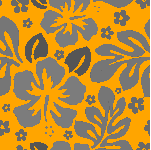
\includegraphics[width=.25\columnwidth]{figs/histograms/b}}}&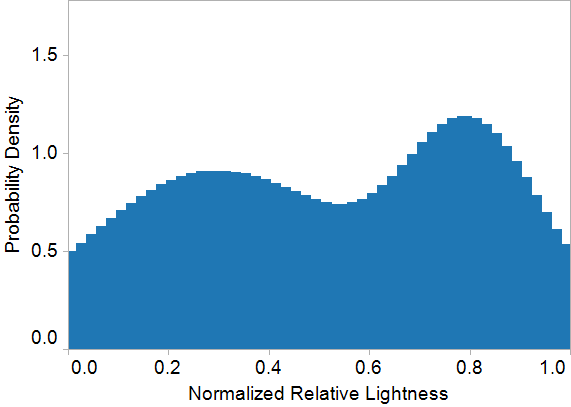
\includegraphics[width=.60\columnwidth]{figs/histograms/backgroundGroupHistogram2}\vspace{0.5em}\\
{\raisebox{4em}{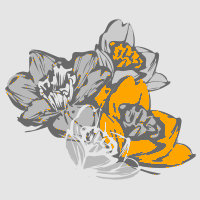
\includegraphics[width=.25\columnwidth]{figs/histograms/f}}}&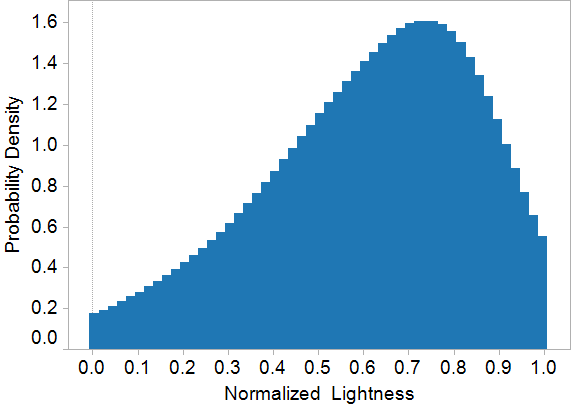
\includegraphics[width=.60\columnwidth]{figs/histograms/foregroundGroupHistogram2}\vspace{0.5em}\\
\end{tabular}

\caption{Predicted distributions over lightness for two different pattern color groups (higlighted in orange). The background has a bimodal distribution, whereas the foreground strictly favors lighter colors.}
\label{fig:unaryHistograms}
\vspace{-1.0em}
\end{figure}

How should we represent these distributions $p$? Closed-form continuous distributions, such as the normal distribution, are appealing for their simplicity.  However, they are unlikely to capture the nuances of data drawn from real patterns, which is often \emph{multimodal} in nature (Figure~\ref{fig:unaryHistograms}).

We adapt the method of Charpiat et al.~\shortcite{MultimodalColorization}, who build multimodal distributions of colors given local texture features for grayscale image colorization. We first discretize the space of possible property values into a finite number of bins. Next, we train a regression model on $(\prop(\colors), \features)$ pairs extracted from the training dataset. The regressor is trained to predict, given a feature vector $\features$, the probability that its corresponding property value $\prop(\colors)$ falls into each bin. Given a new, never-before-seen feature vector, the regressor can then output a \emph{histogram} of these probabilities, one for each property value bin. The histogram is then smoothed using kernel density estimation, and the resulting density forms the final, continuous probability distribution.

In our implementation, we discretize the space of property values using K-means clustering with $k = 10$ on the values found in the training examples. We then use multinomial logistic regression to predict the histograms of property values given features.
%To ensure each pattern template in the training set has equal influence in the regression, we weight each group example by one over the number of groups in the template; segment examples are weighted similarly.
Finally, we smooth the histograms by placing a Gaussian at the center of each histogram bin and setting the Gaussian bandwidth to the average distance to the nearest three other bins~\cite{ThemeEnhancement}.



%Formally, we define a pattern template as $\pattern = (\groups, \segments, \colorVars, \features)$, where $\groups$ is a set of individual color groups $\group$, $\segments$ is a set of individual image segments $\segment$, $\colorVars$ is a set of color variables, and $\features$ is a vector of features extracted from the groups, segments, and adjacent segment pairs within the pattern. Each group $\group$ and segment $\segment$ is associated with a color variable ($\colorVars_\group$ and $\colorVars_\segment$, respectively). All segments within a color group have the same color by definition, so $\colorVars_{\text{group}(\segment)} = \colorVars_\segment$. A coloring $\colors$ is an assignment of colors to color variables. 
%
%As shown in Figure~\ref{fig:ColorCompatOnly}, color compatibility alone does not predict attractive colorings. Good color assignments also depend on the properties of the regions being colored and their spatial arrangement. To capture these dependencies, our model includes spatial terms over groups, segments, and segment adjacencies in the pattern. Group and segment terms capture color dependencies on region features, and segment adjacency terms capture color dependencies on the relationship between nearby regions.
%
%These spatial terms score color assignments based on the conditional probability of a color property $\prop$ (such as lightness or colorfulness) given the features of an object $x$ (which is either a group, segment, or segment adjacency). We compute these probabilities on color properties instead of directly on colors to allow for more generalization over colors that do not occur in the model's training data. For example, Figure~\ref{fig:conditionalDistribution} shows the conditional probability distribution over lightness for the background group of one pattern. The distribution is conditional on several characteristic features of the group, such as its size and the number of segments it contains. In the next sections, we give definitions for the group and segment terms in the model and the adjacency terms. We then describe how to learn these conditional probability distributions from example patterns (Section~\ref{sec:learningPdfs}). A complete listing of the features used, as well as more details on the computation of color properties, can be found in the Appendix.
%
%\begin{figure}[ht]
%\begin{tabular}{cc}
%\raisebox{5em}{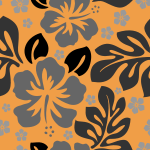
\includegraphics[width=.22\columnwidth]{figs/histogramImage}}&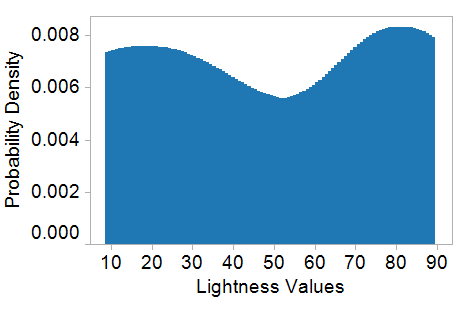
\includegraphics[width=.7\columnwidth]{figs/histogram}%\vspace{0.5em}\\
%\end{tabular}
%\caption{The conditional probability distribution of lightness values for the background color group of a pattern (highlighted in orange). The distribution's multimodality indicates that either very light or very dark backgrounds may be acceptable for this pattern.}
%\label{fig:conditionalDistribution}
%\end{figure}
%
%Both global group features as well as local segment features affect the appearance of a color assignment. The total area of a group and overall spread of its member segments correspond to the overall proportion and spread of its assigned color within an image. In addition, the size and shape of member segments may impact the color a group takes on. As an example, smaller segments may often be more saturated, and a group composed of many small segments may be more likely to be saturated than a group composed of a few small segments but also one large segment \remark{S: Made up example. Should probably find one that holds in our data}.
%
%Our model has one group and one segment term for each of the color properties $ \prop \in \unaryProps$, which are \propName{Lightness}, \propName{Colorfulness}, \propName{NameCounts}, and \propName{NameSaliency}.
%The properties \propName{Lightness} and \propName{Colorfulness} are computed in \lab space. \propName{NameCounts} (counts of how many times a color is described with different names) and \propName{NameSaliency} (how uniquely a color is named) are as described by Heer and Stone~\shortcite{ColorNamingModels}. While lightness and colorfulness capture perceptual properties of color, name saliency and color name counts capture more categorical properties.
%
%The group term for property $\prop \in \unaryProps$ has the statistic:
%\begin{align*}
% \groupTerm(\colors|\pattern) &= \sum_{\group \in \groups} \groupInstStats(\colors_\group | \pattern, \group) \\
% \groupInstStats(\colors_\group | \pattern, \group) &=  \ln p( \prop( \colors_\group ) | \features_\group ) \cdot \size_\group
%\end{align*}
%where $\size_\group$ is the area of the group $\group$ and $\features_\group$ are the features of the group $\group$ (See the Appendix for the complete list of features used). We weight the contribution of each group to the term statistics by its relative area as larger regions tend to have more impact on the appearance of a coloring.
%
%Similarly, the segment term for property $\prop$ has the statistics function $\segTerm(\colors|\pattern) = \sum_{\segment \in \segments} \segInstStats(\colors_\segment | \pattern, \segment)$, where $\segInstStats(\colors_\segment | \pattern, \segment) = \ln p( \prop( \colors_\segment ) | \features_\segment) \cdot \size_\segment$. Here, $\size_\segment$ is the size of the segment $\segment$ and $\features_\segment$ are the features of $\segment$.
%
%These terms contribute unary factors over each color variable by grouping together statistics for the group and segments associated with the variable:
%\begin{align*}
% \factor(\colorVars_\group | \pattern) = \prod_{\prop \in \unaryProps}
% 		\exp( (&\groupTermWeight \cdot \groupInstStats(\colorVars_\group | \pattern, \group)  \\
% 		     + &\segTermWeight \cdot \sum_{\segment \in \group} \segInstStats(\colorVars_\group | \pattern, \segment))) 
%\end{align*}
%
%\subsection{Learning Color Property Distributions}
%\label{sec:learningPdfs}
%
%Each group, segment, and adjacency term requires a conditional probability distribution $p(\prop(\colorVars_x)|\features_x)$ in order to compute its statistic value. What form should these distributions take? Closed-form continuous distributions, such as the normal distribution, are appealing for their simplicity.  However, they are unlikely to capture the nuances of data drawn from real patterns, which is often \emph{multimodal} in nature. As a simple example, pattern backgrounds are typically either very dark or very light (See Figure~\ref{fig:conditionalDistribution}). A normal distribution cannot faithfully capture this type of bimodal behavior.
%
%In our model, we adapt the method of Charpiat et al.~\shortcite{MultimodalColorization}, who learn conditional probability distributions of colors given local texture features for the purpose of grayscale image colorization. This method was designed explicitly to account for multimodality. Our approach is as follows: first, the space of property values is discretized into a finite number of bins. Next, a regressor is trained on pairs of the form $(\prop(\colors_x), \features_x)$ to predict, given a feature vector $\features_x$, the probability that its corresponding property value $\prop(\colors_x)$ falls into each bin. Given a new, never-before-seen feature vector, the regressor can then output a histogram of these probabilities for each bin. The resulting histogram is then smoothed using a form of kernel density estimation, and the resulting density forms the final conditional probability distribution.
%
%We discretize the space of property values using K-means clustering with $k = 10$ on the values found in the training examples. We then use multinomial logistic regression to predict the histograms of property values given features. To ensure each pattern template in the training set has equal influence in the regression, we weight each group example by one over the number of groups in the template; segment and adjacency examples are weighted similarly. Finally, we smooth the histograms using the approach of Wang et al.~\shortcite{ThemeEnhancement}, which places a Gaussian at the center of each histogram bin. To set the Gaussian bandwidth, we use the average distance to the nearest three other bins.